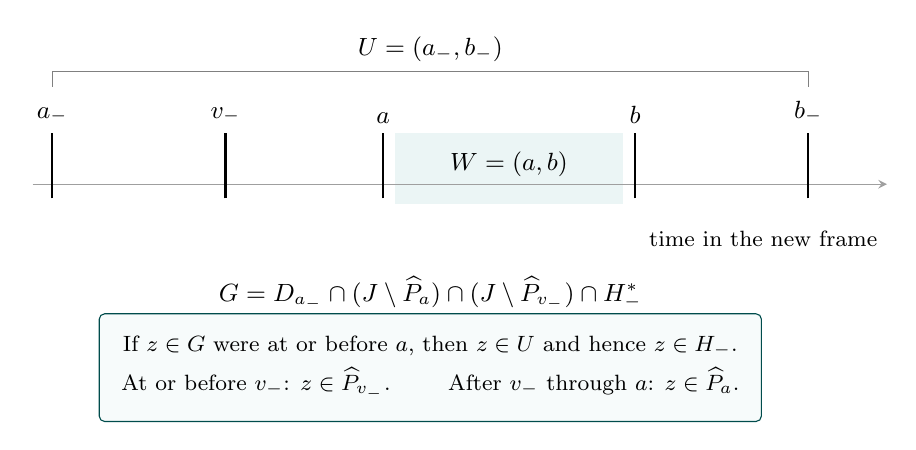
\begin{tikzpicture}[x=1cm,y=1cm,font=\small,>=stealth]
  \fill[teal!8] (4.35,-.25) rectangle (7.25,.65);
  \draw[->,gray!75] (-.25,0) -- (10.6,0);
  \foreach \x in {0,2.2,4.2,7.4,9.6}
    {\draw[thick] (\x,-.18) -- (\x,.65);}
  \node[above] at (0,.65) {$a_-$};
  \node[above] at (2.2,.65) {$v_-$};
  \node[above] at (4.2,.65) {$a$};
  \node[above] at (7.4,.65) {$b$};
  \node[above] at (9.6,.65) {$b_-$};
  \node at (5.8,.25) {$W=(a,b)$};
  \draw[gray] (0,1.24) -- (0,1.43) -- (9.6,1.43) -- (9.6,1.24);
  \node[above] at (4.8,1.43) {$U=(a_-,b_-)$};
  \node[anchor=east,font=\footnotesize] at (10.6,-.7)
    {time in the new frame};
  \node[anchor=north,align=center] at (4.8,-1.05)
    {$G=D_{a_-}\cap (J\setminus\widehat P_a)
      \cap (J\setminus\widehat P_{v_-})\cap H_-^*$};
  \node[draw=teal!60!black,fill=teal!3,rounded corners=2pt,
        inner sep=8pt,align=center,font=\footnotesize] at (4.8,-2.33)
    {If $z\in G$ were at or before $a$, then $z\in U$ and hence $z\in H_-$.\\[3pt]
     At or before $v_-$: $z\in\widehat P_{v_-}$.
     \qquad After $v_-$ through $a$: $z\in\widehat P_a$.};
\end{tikzpicture}
